\special{! TeXDict begin /landplus90{true}store end }

\documentclass[xga]{xdvislides}
\usepackage[landscape]{geometry}
\usepackage{graphics}
\usepackage{graphicx}
\usepackage{colordvi}

\begin{document}
\setfontphv

%%% Headers and footers
\lhead{\slidetitle}                               % default:\lhead{\slidetitle}
\chead{CS615 - Aspects of System Administration}% default:\chead{\relax}
\rhead{Slide \thepage}                       % default:\rhead{\sectiontitle}
\lfoot{\Gray{Writing System Tools}}% default:\lfoot{\slideauthor}
\cfoot{\relax}                               % default:\cfoot{\relax}
\rfoot{\Gray{\today}}

\vspace*{\fill}
\begin{center}
	\Hugesize
		CS615 - Aspects of System Administration\\ [1em]
		Writing System Tools\\ [1em]

	\hspace*{5mm}\blueline\\ [1em]
	\Normalsize
		Department of Computer Science\\
		Stevens Institute of Technology\\
		Jan Schaumann\\
		\verb+jschauma@stevens.edu+\\
		\verb+https://www.cs.stevens.edu/~jschauma/615/+
\end{center}
\vspace*{\fill}

\subsection{Tools}
\vspace*{\fill}
\begin{center}
	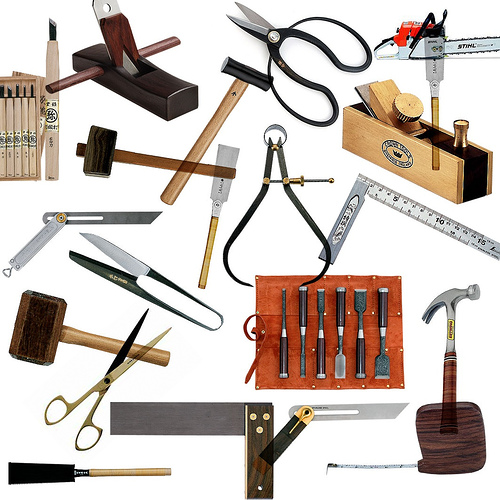
\includegraphics[scale=1.4]{pics/tools.eps}
\end{center}
\vspace*{\fill}

\subsection{Benefits of Automation}
\begin{itemize}
	\item {\em repeatability} -- some of the tasks we
		perform are complex and need to be
		executed in a fixed order
\end{itemize}

\subsection{Benefits of Automation}
\begin{itemize}
	\item {\em repeatability} -- some of the tasks we
		perform are complex and need to be
		executed in a fixed order
	\item {\em reliability} -- we are forgetful, make
		mistakes and tyops, think we know
		better, ...
\end{itemize}

\subsection{Benefits of Automation}
\begin{itemize}
	\item {\em repeatability} -- some of the tasks we
		perform are complex and need to be
		executed in a fixed order
	\item {\em reliability} -- we are forgetful, make
		mistakes and tyops, think we know
		better, ...
	\item {\em regularity} -- some tasks need to
		be executed at a specific time, some with
		a specific frequency, ...
\end{itemize}

\subsection{Benefits of Automation}
\begin{itemize}
	\item {\em repeatability} -- some of the tasks we
		perform are complex and need to be
		executed in a fixed order
	\item {\em reliability} -- we are forgetful, make
		mistakes and tyops, think we know
		better, ...
	\item {\em regularity} -- some tasks need to
		be executed at a specific time, some with
		a specific frequency, ...
	\item {\em flexibility} -- minor variations of
		a complex task or the environment it
		executes in
\end{itemize}


\subsection{Benefits of Automation}
\begin{itemize}
	\item {\em repeatability} -- some of the tasks we
		perform are complex and need to be
		executed in a fixed order
	\item {\em reliability} -- we are forgetful, make
		mistakes and tyops, think we know
		better, ...
	\item {\em regularity} -- some tasks need to
		be executed at a specific time, some with
		a specific frequency, ...
	\item {\em flexibility} -- minor variations of
		a complex task or the environment it
		executes in
\end{itemize}

\vspace{.5in}
Remember the Lego blocks:  Breaking complex tasks
into smaller components allows us to apply these
benefits recursively.

\subsection{Words of Wisdom}
\vspace*{\fill}
\Huge
\begin{center}
Anything you do more than once \\
is worth automating.
\end{center}
\Normalsize
\vspace*{\fill}

\subsection{Who benefits from automation?}
\begin{itemize}
	\item ourselves
	\item our peers
	\item our users
	\item our organization
	\item anybody anywhere
\end{itemize}

\subsection{Evolution of SysAdmin Tools}
\vspace*{\fill}
\begin{center}
	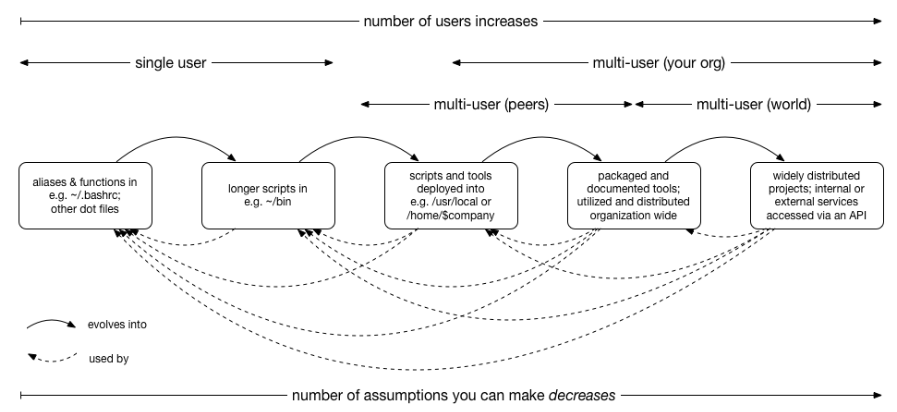
\includegraphics[scale=0.7]{pics/evolution-of-tools.eps}
\end{center}
\vspace*{\fill}

\subsection{Automation Pitfalls}
\begin{itemize}
	\item implementation and debugging takes time and effort
\end{itemize}

\subsection{Automation Pitfalls}
\begin{itemize}
	\item implementation and debugging takes time and effort
	\item automation often increases complexity
\end{itemize}

\subsection{Automation Pitfalls}
\begin{itemize}
	\item implementation and debugging takes time and effort
	\item automation often increases complexity
	\item automation increases the (potential for (negative)) impact
\end{itemize}

\subsection{Automation Pitfalls}
\begin{itemize}
	\item implementation and debugging takes time and effort
	\item automation often increases complexity
	\item automation increases the (potential for (negative)) impact
	\item automation may lead to a loss of audit trail or accountability
\end{itemize}

\subsection{Automation Pitfalls}
\begin{itemize}
	\item implementation and debugging takes time and effort
	\item automation often increases complexity
	\item automation increases the (potential for (negative)) impact
	\item automation may lead to a loss of audit trail or accountability
	\item abstracting a problem requires {\em understanding} it
\end{itemize}


\subsection{Automation Pitfalls}
\begin{itemize}
	\item implementation and debugging takes time and effort
	\item automation often increases complexity
	\item automation increases the (potential for (negative)) impact
	\item automation may lead to a loss of audit trail or accountability
	\item abstracting a problem requires {\em understanding} it
	\item system tools require documentation
\end{itemize}

\subsection{Automation Pitfalls}
\begin{itemize}
	\item implementation and debugging takes time and effort
	\item automation often increases complexity
	\item automation increases the (potential for (negative)) impact
	\item automation may lead to a loss of audit trail or accountability
	\item abstracting a problem requires {\em understanding} it
	\item system tools require documentation
\end{itemize}
\vspace{.5in}
Note: some of these are hidden benefits!


\subsection{Approaching Automation}
Three basic categories:
\\

\begin{itemize}
	\item scripting
	\item programming
	\item software engineering
\end{itemize}

\subsection{Approaching Automation}
Three basic categories:
\\

\begin{itemize}
	\item scripting
		\begin{itemize}
			\item automating {\em very} simple tasks
		\end{itemize}
\end{itemize}

\subsection{Approaching Automation}
Three basic categories:
\\

\begin{itemize}
	\item scripting
		\begin{itemize}
			\item automating {\em very} simple tasks
			\item customization of user environment
		\end{itemize}
\end{itemize}

\subsection{Approaching Automation}
Three basic categories:
\\

\begin{itemize}
	\item scripting
		\begin{itemize}
			\item automating {\em very} simple tasks
			\item customization of user environment
			\item often only suitable for one individual user
		\end{itemize}
\end{itemize}

\subsection{Approaching Automation}
Three basic categories:
\\

\begin{itemize}
	\item scripting
		\begin{itemize}
			\item automating {\em very} simple tasks
			\item customization of user environment
			\item often only suitable for one individual user
			\item usually eventually evolves into larger programs
		\end{itemize}
\end{itemize}


\subsection{Approaching Automation}
Three basic categories:
\\
\begin{itemize}
	\item scripting
		\begin{itemize}
			\item automating {\em very} simple tasks
			\item customization of user environment
			\item often only suitable for one individual user
			\item usually eventually evolves into larger programs
		\end{itemize}
	\item programming
		\begin{itemize}
			\item suitable for simple to moderately complex tasks
		\end{itemize}
\end{itemize}

\subsection{Approaching Automation}
Three basic categories:
\\

\begin{itemize}
	\item scripting
		\begin{itemize}
			\item automating {\em very} simple tasks
			\item customization of user environment
			\item often only suitable for one individual user
			\item usually eventually evolves into larger programs
		\end{itemize}
	\item programming
		\begin{itemize}
			\item suitable for simple to moderately complex tasks
			\item results frequently used by a small base of users
		\end{itemize}
\end{itemize}

\subsection{Approaching Automation}
Three basic categories:
\\

\begin{itemize}
	\item scripting
		\begin{itemize}
			\item automating {\em very} simple tasks
			\item customization of user environment
			\item often only suitable for one individual user
			\item usually eventually evolves into larger programs
		\end{itemize}
	\item programming
		\begin{itemize}
			\item suitable for simple to moderately complex tasks
			\item results frequently used by a small base of users
			\item uses basic framework or common toolkits
		\end{itemize}
\end{itemize}

\subsection{Approaching Automation}
Three basic categories:
\\

\begin{itemize}
	\item scripting
		\begin{itemize}
			\item automating {\em very} simple tasks
			\item customization of user environment
			\item often only suitable for one individual user
			\item usually eventually evolves into larger programs
		\end{itemize}
	\item programming
		\begin{itemize}
			\item suitable for simple to moderately complex tasks
			\item results frequently used by a small base of users
			\item uses basic framework or common toolkits
			\item provides consistent interface
		\end{itemize}
\end{itemize}

\subsection{Approaching Automation}
Three basic categories:
\\

\begin{itemize}
	\item scripting
		\begin{itemize}
			\item automating {\em very} simple tasks
			\item customization of user environment
			\item often only suitable for one individual user
			\item usually eventually evolves into larger programs
		\end{itemize}
	\item programming
		\begin{itemize}
			\item suitable for simple to moderately complex tasks
			\item results frequently used by a small base of users
			\item uses basic framework or common toolkits
			\item provides consistent interface
			\item may evolve into full product
		\end{itemize}
\end{itemize}


\subsection{Approaching Automation}
Three basic categories:
\\

\begin{itemize}
	\item software development
		\begin{itemize}
			\item required for any reasonably complex task
		\end{itemize}
\end{itemize}

\subsection{Approaching Automation}
Three basic categories:
\\

\begin{itemize}
	\item software development
		\begin{itemize}
			\item required for any reasonably complex task
			\item uses formal software engineering approach (measurable goals,
				requirements, specifications, ...)
		\end{itemize}
\end{itemize}

\subsection{Approaching Automation}
Three basic categories:
\\

\begin{itemize}
	\item software development
		\begin{itemize}
			\item required for any reasonably complex task
			\item uses formal software engineering approach (measurable goals,
				requirements, specifications, ...)
			\item may evolve from previous prototypes
		\end{itemize}
\end{itemize}


\subsection{Approaching Automation}
Three basic categories:
\\

\begin{itemize}
	\item software development
		\begin{itemize}
			\item required for any reasonably complex task
			\item uses formal software engineering approach (measurable goals,
				requirements, specifications, ...)
			\item may evolve from previous prototypes
			\item requires ongoing continous maintenance / development efforts
		\end{itemize}
\end{itemize}


\subsection{The right tool?}
\vspace*{\fill}
\begin{center}
	
\includegraphics[scale=0.6]{pics/hammer.eps}
\end{center}
\vspace*{\fill}

\subsection{Picking the right tool}
Make sure to understand your requirements:

\begin{itemize}
	\item motivation / goals
	\item target audience
	\item scope
	\item dependencies
	\item input / output requirements and contraints
\end{itemize}


\subsection{The right tool?}
Bourne shell (/bin/sh) \\

\begin{itemize}
	\item lowest common denominator
	\item available and reliable on most platforms (but beware of non-portable
		bash(1) "enhancements")
	\item beware of "quick-and-dirty" solutions, they grow to become
		unmaintainable
	\item treat shell as any other programming language:
		\begin{itemize}
			\item use functions
			\item use suitably scoped variables
			\item follow Unix philosophy
			\item properly package your tool
		\end{itemize}
\end{itemize}

Note: you {\em can} ``program'' in shell, building complex
systems.


\subsection{The right tool?}
Perl, Python, Ruby, Node, ... \\

\begin{itemize}
	\item suitable for moderately complex tasks
	\item move to these when sed(1), awk(1), etc. become too cumbersome
	\item text manipulation frequently easier
	\item beware of "quick-and-dirty" solutions, they grow to become
		unmaintainable
	\item try to build self-contained modules that can be tested independent of
		the "main" program
	\item wealth of libraries available -- use them! (And remember to explicitly
		require them.)
	\item properly package your tool
\end{itemize}

Note: LOC is not a direct indicator of duct-tapeness.

\subsection{The right tool?}
Perl, PHP, Tcl, JavaScript, CoffeeScript, ... \\

\begin{itemize}
	\item http/web server interfaces
	\item CGI "scripts" / server-side execution
	\item interface with/utilize APIs in a specific domain/vendor products
	\item frequent cause of all sorts of security problems due to interface with
		user data / exposure on the internet
\end{itemize}

\subsection{The right tool?}
C, C++, Go, ... \\

\begin{itemize}
	\item performance benefits
	\item portability
	\item sufficient low-levelness
	\item systems understanding
	\item fix/patch your other tools / the system
\end{itemize}

\subsection{Interpreted Languages}
General advantages: \\

\begin{itemize}
	\item short development cycle
	\item normally facilitate things like string manipulation, arithmetic and
		more complex regular expressions
	\item easily handle multiple file handles and other I/O
	\item some security features
	\item tens of thousands of special- and general-purpose modules available
\end{itemize}

\subsection{Interpreted Languages}
General Disadvantages: \\

\begin{itemize}
	\item no one tool fits all purposes
	\item tens of thousands of special- and general-purpose modules available $=>$
		lots of duplication, stale code, questionable quality \\
		packaging and dependency resolution nightmares
	\item security features frequently neglected or circumvented ("too hard" or
		more precisely "inconvenient")
	\item everybody has their particular favorite (and dislikes one or the
		other)
	\item interpreter not (necessarily) universally available / installed
\end{itemize}


% % \subsection{Repeating Jobs}
% % Humans are terrible at remembering to do something repeatedly and
% % regularly.  We should let computers do that. \\
% % 
% % \vspace{.5in}
% % 
% % Enter \verb+cron(8)+ / \verb+crontab(5)+.
% % 
% % \subsection{Repeating Jobs}
% % Example: \\
% % \vspace{.5in}
% % 
% % \begin{verbatim}
% % 30 2 * * 7 find /tmp -type f -mtime +7 -atime +7 -exec rm -f '{}' ';'
% % \end{verbatim}
% % 
% % \subsection{Time is relative}
% % Sometimes an hour doesn't exist. \\
% % 
% % \vspace{.5in}
% % Sometimes an hour repeats. \\
% % 
% % \vspace{.5in}
% % What happens to your \verb+crontab+?
% % \begin{verbatim}
% % 30 2 * * 7 find /tmp -type f -mtime +7 -atime +7 -exec rm -f '{}' ';'
% % \end{verbatim}
% % 
% % \subsection{Time is relative}
% % Sometimes an hour doesn't exist. \\
% % 
% % \vspace{.5in}
% % Sometimes an hour repeats. \\
% % 
% % \vspace{.5in}
% % All sorts of other things you thought were true are not: \\
% % \verb+http://infiniteundo.com/post/25326999628/falsehoods-programmers-believe-about-time+
% % 
% % \subsection{Regular Expressions 101}
% % A {\em regular expression} is a pattern that describes a set of strings. \\
% % 
% % \begin{itemize}
% % 	\item patterns can be
% % 		\begin{itemize}
% % 			\item single characters (\verb+a+)
% % 			\item a bracket expression, such as
% % 				\begin{itemize}
% % 					\item a set of characters -- \verb+[aK2l,]+
% % 					\item a range expression -- \verb+[a-z]+
% % 					\item a negated bracket expression -- \verb+[^0-9]+
% % 				\end{itemize}
% % 			\item a character with a special meaning, such as
% % 				\begin{itemize}
% % 					\item \verb+.+ -- any single character
% % 					\item \verb+^+ -- beginning of line
% % 					\item \verb+$+ -- end of line
% % 				\end{itemize}
% % 			\item a combination of patterns
% % 		\end{itemize}
% % \end{itemize}
% % 
% % \subsection{Regular Expressions}
% % \begin{itemize}
% % 	\item patterns can be followed by qualifiers and quantifiers
% % 		\begin{itemize}
% % 			\item \verb+?+ -- the pattern is optional and matched at most once
% % 			\item \verb+*+ -- the pattern will be matched zero or more times
% % 			\item \verb|+| -- the pattern will be matched one or more times
% % 			\item \verb+{n}+ -- the pattern is matched exactly \verb+n+ times
% % 			\item \verb+{n,}+ -- the pattern is matched \verb+n+ or more times
% % 			\item \verb+{n,m}+ -- the pattern is matched at least \verb+n+,
% % 				but no more than \verb+m+ times
% % 		\end{itemize}
% % 	\item patterns can be logically grouped together \verb+(1[a-z]2|a[0-9]z)+
% % 	\item matched patterns can be remembered and referenced lateron
% % \end{itemize}
% % \addvspace{.5in}
% % NB: different tools/libraries implement regular expressions somewhat differently

\subsection{Regular Expressions}
Example exercises:
\begin{itemize}
	\item check if a string is a valid date \\
		\verb+03/07/2016, 7.3.2016, 2016-03-07, 2016/03/07, ...+
	\item check if a string is a valid IPv4 address \\
		\verb+0.0.0.0, 255.255.255.255, ...+
	\item check if a string is a valid IPv6 address \\
		\verb+::1, fe80::e276:63ff:fe72:3900%xennet0, 2001:470:30:84:e276:63ff:fe72:3900, ...+
	\item extract all URLs from a document \\
		\verb+http://example.com, ftp://example.com/dir/file.html,+ \\
		\verb+https://example.com/?foo=bar&blob=';alert(1);,+ \\
		\verb+http://example.com/?redir=http://example.com, ...+
	\item extract all proper words from a document \\
		\verb+word, it's, Name, Henry the 3rd, cross-site scripting, ...+
\end{itemize}

\subsection{Regular Expressions}
IPv4:

\subsection{Regular Expressions}
IPv4:
\begin{verbatim}
(25[0-5]|2[0-4][0-9]|[01]?[0-9][0-9]?)\.(25[0-5]|2[0-4][0-9]|[01]?
[0-9][0-9]?)\.(25[0-5]|2[0-4][0-9]|[01]?\.(25[0-5]|2[0-4][0-9]|[01]
?[0-9][0-9]?)\.(25[0-5]|2[0-4][0-9]|[01]?[0-9][0-9]?)
\end{verbatim}

\subsection{Regular Expressions}
IPv4:
\begin{verbatim}
(25[0-5]|2[0-4][0-9]|[01]?[0-9][0-9]?)\.(25[0-5]|2[0-4][0-9]|[01]?
[0-9][0-9]?)\.(25[0-5]|2[0-4][0-9]|[01]?\.(25[0-5]|2[0-4][0-9]|[01]
?[0-9][0-9]?)\.(25[0-5]|2[0-4][0-9]|[01]?[0-9][0-9]?)
\end{verbatim}

IPv6:
\begin{verbatim}
(([0-9a-fA-F]{1,4}:){7,7}[0-9a-fA-F]{1,4}|([0-9a-fA-F]{1,4}:){1,7}:|
([0-9a-fA-F]{1,4}:){1,6}:[0-9a-fA-F]{1,4}|([0-9a-fA-F]{1,4}:){1,5}(:
[0-9a-fA-F]{1,4}){1,2}|([0-9a-fA-F]{1,4}:){1,4}(:[0-9a-fA-F]{1,4}){1
,3}|([0-9a-fA-F]{1,4}:){1,3}(:[0-9a-fA-F]{1,4}){1,4}|([0-9a-fA-F]{1,
4}:){1,2}(:[0-9a-fA-F]{1,4}){1,5}|[0-9a-fA-F]{1,4}:((:[0-9a-fA-F]{1,
4}){1,6})|:((:[0-9a-fA-F]{1,4}){1,7}|:)|fe80:(:[0-9a-fA-F]{0,4}){0,4
}%[0-9a-zA-Z]{1,}|::(ffff(:0{1,4}){0,1}:){0,1}((25[0-5]|(2[0-4]|1{0,
1}[0-9]){0,1}[0-9])\.){3,3}(25[0-5]|(2[0-4]|1{0,1}[0-9]){0,1}[0-9])|
([0-9a-fA-F]{1,4}:){1,4}:((25[0-5]|(2[0-4]|1{0,1}[0-9]){0,1}[0-9])\.
){3,3}(25[0-5]|(2[0-4]|1{0,1}[0-9]){0,1}[0-9]))
\end{verbatim}

\subsection{Regular Expressions}
{\em Some people, when confronted with a problem,
think "I know, I'll use regular expressions." Now they
have two problems.} \\

Better:
\begin{verbatim}
        if (inet_pton(AF_INET, $ip)) {
                # AF_INET
        } elsif (inet_pton(AF_INET6, $ip)) {
                # AF_INET6
        } else {
                # not an IP address
        }
\end{verbatim}

Know when you need to be precise, and when 'good
enough' is good enough.

% % \subsection{Example exercises}
% % Page view statistics for Wikimedia projects \\
% % {\tt http://dumps.wikimedia.org/other/pagecounts-all-sites/} \\
% % {\tt https://wikitech.wikimedia.org/wiki/Analytics/Data/Pagecounts-all-sites} \\
% % \vspace{.5in}
% % 
% % On {\tt linux-lab.cs.stevens.edu}:
% % \begin{verbatim}
% % ls -l ~jschauma/public_html/615/pagecounts-20160301-000000
% % \end{verbatim}
% % \vspace{.5in}
% % Format: \\
% % \verb+    domain page_title count_views total_response_size+
% % 
% % \subsection{Example exercises}
% % \begin{verbatim}
% % ls -l ~jschauma/public_html/615/pagecounts-20160301-000000
% % \end{verbatim}
% % Format: \\
% % \verb+    domain page_title count_views total_response_size+
% % \\
% % 
% % How many unique objects were requested? \\
% % 
% % How many unique objects were requested for {\tt en} only? \\
% % 
% % Which is the most often requested object? \\
% % 
% % How many requests per second were handled during this hour? \\
% % 
% % How much data was transferred in total? \\
% % 
% % Which was the largest object requested?
% % 
% % \subsection{Example exercises}
% % What is the longest word found on the ten most frequently retrieved
% % English Wikipedia pages?
% % 
% % \begin{verbatim}
% % for f in $(grep -i "^en " ${FILE}| sort -k3 -n | tail -10 |
% %         sed -e 's/en \(.*\) [0-9]* [0-9]*/\1/'); do
% %         links -dump http://en.wikipedia.org/wiki/${f}
% % done |
% % tr '[:punct:]' ' ' |
% % tr '[:space:]' '\n' |
% % tr '[:upper:]' '[:lower:]' |
% % egrep '^[a-z]+$' |
% % awk '{ print length() " " $0; }' |
% % sort |
% % uniq |
% % sort -n |
% % tail -1
% % \end{verbatim}

\newpage
\vspace*{\fill}
\begin{center}
    \Hugesize
        Hooray! \\ [1em]
    \hspace*{5mm}
    \blueline\\
    \hspace*{5mm}\\
        5 Minute Break
\end{center}
\vspace*{\fill}

\subsection{User Interface}
\\
\vspace*{\fill}
\begin{center}
	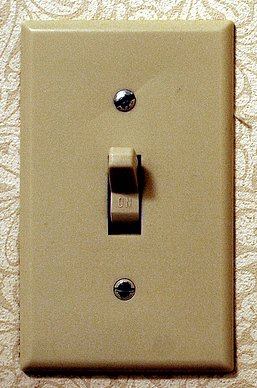
\includegraphics[scale=3]{pics/switch.eps}
\end{center}
\vspace*{\fill}


\subsection{Unix Philosophy}
\\
\Huge
\begin{center}
	Write programs that do one thing and do it well.\\
	\vspace{.5in}
	Write programs to work together. \\
	\vspace{.5in}
	Write programs to handle text streams, because that is a universal interface.
\end{center}
\Normalsize

\subsection{Be Boring}
\\
\Huge
\begin{center}
	Use boring technology. \\
\vspace{1in}
	Write boring code.
\end{center}
\Normalsize

\subsection{Know your languages / eco-system}
Some advice transcends language: \\

\begin{verbatim}
$ echo import this | python
\end{verbatim}

\subsection{The Zen of Python}
\Huge
\begin{center}
Beautiful is better than ugly.
\end{center}

\subsection{The Zen of Python}
\begin{center}
Explicit is better than implicit.
\end{center}

\subsection{The Zen of Python}
\begin{center}
    Simple is better than complex.
\vspace*{\fill}
	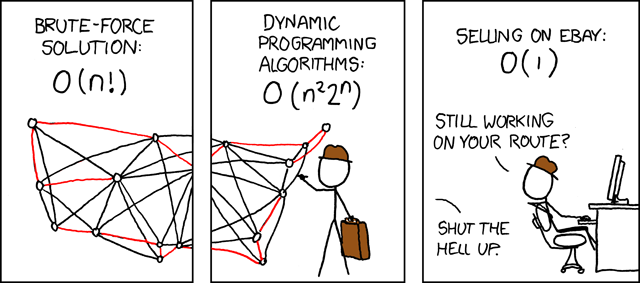
\includegraphics[scale=0.8]{pics/complexity.eps}
	\\
	\small \verb+http://xkcd.com/399/+
\end{center}
\vspace*{\fill}
\Huge

\subsection{The Zen of Python}
\begin{center}
    Complex is better than complicated.
\end{center}

\subsection{The Zen of Python}
\begin{center}
    Flat is better than nested. \\
    Sparse is better than dense. \\
\vspace{.5in}
    Readability counts.
\end{center}

\subsection{A comment on comments}
Write descriptive code, use descriptive variables and
function names. \\
\vspace{1in}

Comments should explain {\em why}, not {\em what}. \\

\subsection{The Zen of Python}
\begin{center}
    Special cases aren't special enough to break the rules.
\end{center}

\subsection{The Zen of Python}
\begin{center}
    Special cases aren't special enough to break the rules. \\
\addvspace{.5in}
    Although practicality beats purity.
\end{center}

\subsection{The Zen of Python}
\\
\begin{center}
    Errors should never pass silently.
\end{center}

\subsection{The Zen of Python}
\\
\begin{center}
    Errors should never pass silently. \\
\addvspace{.2in}
	\small
	(That would be implicitly accepted failure.)
\end{center}
\Huge

\subsection{The Zen of Python}
\\
\begin{center}
    Errors should never pass silently. \\
\addvspace{.2in}
	\small
	(That would be implicitly accepted failure.) \\
\addvspace{.2in}
	(You know what would be better than something {\em implicit}?)
\end{center}

\subsection{The Zen of Python}
\\
\begin{center}
    Errors should never pass silently. \\
\addvspace{.2in}
	\small
	(That would be implicitly accepted failure.) \\
\addvspace{.2in}
	(You know what would be better than something {\em implicit}?) \\
\addvspace{.2in}
	(Why, of course, something {\em explicit}!)
\end{center}

\subsection{The Zen of Python}
\\
\begin{center}
    Errors should never pass silently. \\
\addvspace{.5in}
    Unless explicitly silenced.
\end{center}

\subsection{The Zen of Python}
\begin{center}
    In the face of ambiguity, refuse the temptation to guess.
\end{center}

\subsection{The Zen of Python}
\begin{center}
    There should be one -- and preferably only one -- obvious way to do it.
\end{center}

\subsection{The Zen of Python}
\begin{center}
    There should be one -- and preferably only one -- obvious way to do it.

\addvspace{.5in}

    Although that way may not be obvious at first unless you're Dutch. \\
% You have to understand the idiomatic way to do
% things.
\end{center}


\subsection{The Zen of Python}
\begin{center}
    Now is better than never.
\end{center}

\subsection{The Zen of Python}
\begin{center}
    Now is better than never.  \\

\addvspace{.5in}

    Although never is often better than *right* now.
\end{center}

\subsection{The Zen of Python}
\begin{center}
    If the implementation is hard to explain, \\
it's a bad idea.
\end{center}

\subsection{The Zen of Python}
\begin{center}
    If the implementation is easy to explain, \\
	it {\em may} be a good idea.
\end{center}

\subsection{A simple interface, easy to explain.  Yet...}
\\
\vspace*{\fill}
\begin{center}
	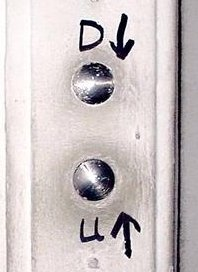
\includegraphics[scale=1.0]{pics/elevator_buttons-reverse.eps}
\end{center}
\vspace*{\fill}


\subsection{The Zen of Python}
\begin{center}
    Namespaces are one honking great idea -- let's do more of those!
\end{center}
\Normalsize

\subsection{Documentation}
\vspace*{\fill}
\begin{center}
	\includegraphics[scale=0.9]{pics/manual.eps}
	\hspace{.5in}
	\includegraphics[scale=0.9]{pics/manual2.eps}
	\\
	\vspace{.2in}
	\Huge
	{\bf WTFM}
	\Normalsize
\end{center}
\vspace*{\fill}

\subsection{Robustness Principle or Postel's Law}
\\
\Huge
\begin{center}
	Be conservative in what you do; be liberal in what you accept from others.
\end{center}
\Normalsize


\subsection{POLA}
Principle of Least Astonishment
\\
\vspace*{\fill}
\begin{center}
	
\includegraphics[scale=0.7]{pics/kinder-surprise.eps}
\end{center}
\vspace*{\fill}

\subsection{Know your Users}
Who will use your tools?
\begin{itemize}
	\item you yourself only
	\item your peers
	\item your "users"
	\item anybody else
\end{itemize}
\vspace{.5in}
What assumptions can you make? \\
How will your users script around your tool?

\subsection{Avoid the Quick Fix}
\\
\Huge
\begin{center}
There's nothing as permanent \\
as a temporary solution.
\end{center}
\Normalsize

\subsection{Avoid the Project That Was Never Finished}
\\
\Huge
\begin{center}
	Don't let the Perfect be the enemy of the Good.
\end{center}
\Normalsize

\subsection{Avoid Feature Creep}
\vspace*{\fill}
\begin{center}
	
\includegraphics[scale=1.0]{pics/feeping.eps} \\
	\small
	\verb+http://www.feepingcreatures.com+
\end{center}
\vspace*{\fill}

\subsection{Release Early, Release Often}
\\
\Huge
\begin{center}
	``More users find more bugs.'' \\
	\addvspace{.2in}
	\small F. Brooks, ``The Mythical Man Month''
\end{center}
\Normalsize

\subsection{Take a good look in the mirror!}
\\
\vspace*{\fill}
\begin{center}
	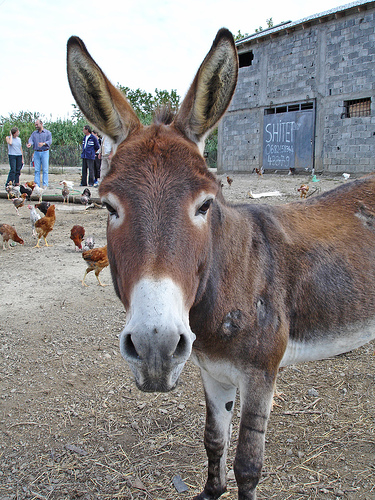
\includegraphics[scale=0.65]{pics/donkey.eps} \\
	\small
	Looks like {\em you} are the ass.
\end{center}
\vspace*{\fill}

\subsection{Learn to write a detailed bug report}
Pre-requisite:
\begin{itemize}
	\item RTFM
	\item Internet Search
	\item Know Your Community
\end{itemize}

\subsection{Learn to write a detailed bug report}
Pre-requisite: Do your homework. \\

Required:
\begin{itemize}
	\item Description Of Problem
	\item Steps To Reproduce
	\item Expected Results
	\item Actual Results
\end{itemize}

\subsection{Learn to write a detailed bug report}
Pre-requisite: Do your homework. \\

Required:
\begin{itemize}
	\item Description Of Problem
	\item Steps To Reproduce
	\item Expected Results
	\item Actual Results
\end{itemize}
\vspace{.125in}

Optional / recommended:
\begin{itemize}
	\item Screenshots / {\em exact} copy of terminal I/O ({\tt script(1)})
	\item Suggested Remediation
	\item Code Patch
\end{itemize}

\subsection{Know how to use your ticket tracking system!}
\begin{itemize}
	\item {\em value} problem reports
	\item link related tickets
	\item have a backlog strategy
	\item understand the lifetime of a ticket \\
		(reported, accepted, assigned, resolved, closed)
	\item abstain from passive-aggressive ticket
		closing and re-opening
\end{itemize}

\subsection{Increase the Bus Factor}
\vspace*{\fill}
\begin{center}
	\includegraphics[scale=0.85]{pics/bert-ernie.eps} \\
	\small
	``Just friends.''
\end{center}
\vspace*{\fill}

\subsection{Collaboration is non-optional}
Efficient use of Version Control Systems is a
requirement.  They allow you to:

\begin{itemize}
        \item collaborate with others
        \item simultaneously work on a code base
        \item keep old versions of files
        \item keep a log of the who, when, what, and why of any changes
        \item perform release engineering by creating {\em branches}
\end{itemize}

\subsection{Commit Messages}

Commit messages are like comments: often useless and
misleading, but critical in understanding human
thinking behind the code. \\

Commit messages are full sentences in correct and
properly formatted English.
\\

Commit messages briefly summarize the {\em what}, but
provide important historical context as to the {\em
how} and, more importantly, {\em why}. \\

Commit messages SHOULD reference and integrate with
ticket tracking systems. \\

See also:
\begin{itemize}
        \item \verb+https://is.gd/Wd1LhA+
        \item \verb+https://is.gd/CUtwhA+
        \item \verb+https://is.gd/rPQj5E+
\end{itemize}


\subsection{Fix Broken Windows}
\vspace*{\fill}
\begin{center}
	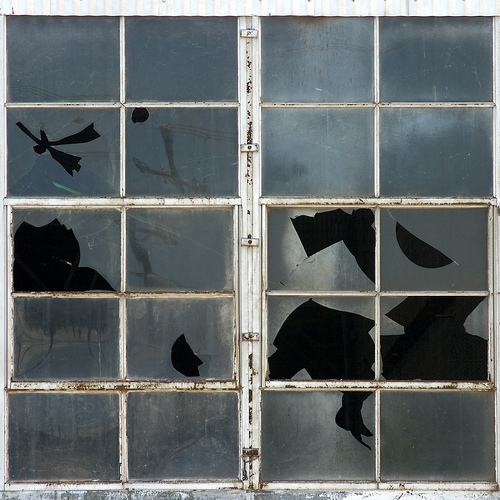
\includegraphics[scale=0.6]{pics/broken-windows.eps}
\end{center}
\vspace*{\fill}

\subsection{Scope}
\\
\Huge
\begin{center}
	``Contraints are friends.'' \\
	\addvspace{.2in}
	\small F. Brooks, ``The Mythical Man Month''
\end{center}
\Normalsize


\subsection{Scalability}
\begin{itemize}
	\item Simplify!
\end{itemize}

\subsection{Scalability}
\begin{itemize}
	\item Simplify!
	\item Reduce or eliminate interactions with the user.
\end{itemize}

\subsection{Scalability}
\begin{itemize}
	\item Simplify!
	\item Reduce or eliminate interactions with the user.
	\item Premature optimization is the root of all evil.
\end{itemize}

\subsection{Scalability}
\begin{itemize}
	\item Simplify!
	\item Reduce or eliminate interactions with the user.
	\item Premature optimization is the root of all evil.
	\item So is excusing shoddy programming.
\end{itemize}

\subsection{Scalability}
\begin{itemize}
	\item Simplify!
	\item Reduce or eliminate interactions with the user.
	\item Premature optimization is the root of all evil.
	\item So is excusing shoddy programming.
	\item Fix {\em all} warnings and errors.
\end{itemize}

\subsection{Scalability}
\begin{itemize}
	\item Simplify!
	\item Reduce or eliminate interactions with the user.
	\item Premature optimization is the root of all evil.
	\item So is excusing shoddy programming.
	\item Fix {\em all} warnings and errors.
	\item Document all assumptions.  Be specific.
\end{itemize}

\subsection{Scalability}
\begin{itemize}
	\item Simplify!
	\item Reduce or eliminate interactions with the user.
	\item Premature optimization is the root of all evil.
	\item So is excusing shoddy programming.
	\item Fix {\em all} warnings and errors.
	\item Document all assumptions.  Be specific.
	\item Always apply the Principle of Least Privilege.
\end{itemize}

\subsection{Scalability}
\begin{itemize}
	\item Simplify!
	\item Reduce or eliminate interactions with the user.
	\item Premature optimization is the root of all evil.
	\item So is excusing shoddy programming.
	\item Fix {\em all} warnings and errors.
	\item Document all assumptions.  Be specific.
	\item Always apply the Principle of Least Privilege.
	\item Assume hostile input and usage.
\end{itemize}

\subsection{Scalability}
\begin{itemize}
	\item Simplify!
	\item Reduce or eliminate interactions with the user.
	\item Premature optimization is the root of all evil.
	\item So is excusing shoddy programming.
	\item Fix {\em all} warnings and errors.
	\item Document all assumptions.  Be specific.
	\item Always apply the Principle of Least Privilege.
	\item Assume hostile input and usage.
	\item Understand your code.
\end{itemize}

\subsection{Scalability}
\begin{itemize}
	\item Simplify!
	\item Reduce or eliminate interactions with the user.
	\item Premature optimization is the root of all evil.
	\item So is excusing shoddy programming.
	\item Fix {\em all} warnings and errors.
	\item Document all assumptions.  Be specific.
	\item Always apply the Principle of Least Privilege.
	\item Assume hostile input and usage.
	\item Understand your code.
	\item Document your tools.
\end{itemize}


\subsection{Program Maintenance}
\\
\Huge
\begin{center}
	``... is an entropy-increasing process, and even its most skillful
	execution only delays the subsidence of the system into unfixable
	obsolescence.'' \\
	\addvspace{.2in}
	\small F. Brooks, ``The Mythical Man Month''
\end{center}
\Normalsize

\subsection{Toss it!}
\vspace*{\fill}
\begin{center}
	
\includegraphics[scale=3]{pics/waste.eps}
\end{center}
\vspace*{\fill}

\subsection{HW}
\vspace{.5in}
\begin{center}
\begin{verbatim}
https://www.cs.stevens.edu/~jschauma/615/s18-hw5.html
\end{verbatim}
\end{center}

\subsection{That's All, Folks!}
\vspace*{\fill}
\Huge
\begin{center}
Go away or I \\
will replace you \\
with a very small \\
shell script.
\end{center}
\Normalsize
\vspace*{\fill}


\subsection{Reading}
Shell:
\begin{itemize}
	\item \verb+http://www.tldp.org/HOWTO/Bash-Prog-Intro-HOWTO.html+
	\item \verb+http://www.tldp.org/LDP/abs/html/+
	\item \verb+http://sed.sourceforge.net/sed1line.txt+
	\item \verb+csh(1)+, \verb+ksh(1)+, \verb+sh(1)+
\end{itemize}
Perl:
\begin{itemize}
	\item \verb+http://www.perl.com+
	\item \verb+http://www.cpan.org+
	\item \verb+perl(1)+, \verb+perldoc(1)+,
	\verb+perlfaq(1)+
\end{itemize}
Python:
\begin{itemize}
	\item \verb+http://www.python.org+
	\item pydoc
\end{itemize}

\subsection{Reading}
Ruby:
\begin{itemize}
	\item \verb+http://www.ruby-lang.org/en/+
	\item \verb+http://is.gd/cE7iFR+
	\item \verb+http://is.gd/DR4aNU+
\end{itemize}

Other:
\begin{itemize}
	\item \verb+http://www.regex.alf.nu/+
	\item \verb+http://is.gd/jDDGpW+
	\item \verb+https://www.netmeister.org/blog/writing-tools.html+
\end{itemize}

\end{document}
